% aspec ratio of slides
\documentclass[aspectratio=43, notes]{beamer} 	% 4:3 Format
%\documentclass[aspectratio=169]{beamer} % 16:9 Format

% load packages
% Paket für Deutsche Sprache (Übersetzungen von Chapter zu Kapitel, 
% richtige Umlaute, richtige % Silbentrennung)
% siehe auch http://de.wikipedia.org/wiki/Babel-System
\usepackage[english]{babel}

% Eingabecodierung, deutsche Umlaute oder die akzentuierten Zeichen sind verfügbar 
% und können direkt eingegeben werden
% siehe auch http://de.wikipedia.org/wiki/UTF8
\usepackage[utf8]{inputenc}

% Ausgabeschriftart von LaTeX festlegen
% siehe auch http://de.wikibooks.org/wiki/LaTeX-Schnellkurs:_Erste_Schritte
\usepackage[T1]{fontenc}

% Standardpfad für Grafiken
\graphicspath{{logos/}{bilder/}}

% Paket zum Erstellen von Plots mit TikZ
\usepackage{pgfplots}
% immer die neueste Version benutzen
\pgfplotsset{compat=newest}
% Verbindung von Linien durch eine schräge Kante
\pgfplotsset{every axis/.append style={line join=bevel}}
% Formatvorlage für Präsentationen
\mode<beamer>{
	\pgfplotsset{
		beamer/.style={
			width=0.8\textwidth,
			height=0.45\textwidth,
			legend style={font=\scriptsize},
			tick label style={font=\footnotesize},
			label style={font=\small},
			max space between ticks=28,
		}
	}
}
\mode<handout>{
	\pgfplotsset{
		beamer/.style={
			width=0.8\textwidth,
			height=0.45\textwidth,
			legend style={font=\scriptsize},
			tick label style={font=\footnotesize},
			label style={font=\small},
			max space between ticks=25,
		}
	}
}
\mode<article>{
	\pgfplotsset{
		beamer/.style={
			width=0.8\textwidth,
			height=0.45\textwidth,
			max space between ticks=35,
		}
	}
}
% neue Größenvorlage für zwei Plots nebeneinander anlegen
\pgfplotsset{
	scriptsize/.style={
		width=0.34\textwidth,
		height=0.1768\textwidth,
		legend style={font=\scriptsize},
		tick label style={font=\scriptsize},
		label style={font=\footnotesize},
		title style={font=\footnotesize},
		every axis title shift=0pt,
		max space between ticks=25,
		every mark/.append style={mark size=7},
		major tick length=0.1cm,
		minor tick length=0.066cm,
	}
}
\pgfplotsset{
	small/.style={
		width=6.5cm,
		height=,
		tick label style={font=\footnotesize},
		label style={font=\small},
		legend style={font=\footnotesize},
		max space between ticks=30,
	}
}
% Legendeneintrage standardmäßig links ausrichten
\pgfplotsset{legend cell align=left}
% Hauptgitternetz zeichnen
\pgfplotsset{xmajorgrids}
\pgfplotsset{ymajorgrids}
% Anzahl der kleinen Teilstriche zwischen zwei großen Teilstrichen
%\pgfplotsset{minor x tick num={3}}
%\pgfplotsset{minor y tick num={3}}
% feines Gitternetz zeichnen
%\pgfplotsset{xminorgrids}
%\pgfplotsset{yminorgrids}
% nur nach den Achsen skalieren
\pgfplotsset{scale only axis}
% Farben wie in MATLAB definieren
\definecolor{matlab1}{rgb}{0,0,1}
\definecolor{matlab2}{rgb}{0,0.5,0}
\definecolor{matlab3}{rgb}{1,0,0}
\definecolor{matlab4}{rgb}{0,0.75,0.75}
\definecolor{matlab5}{rgb}{0.75,0,0.75}
\definecolor{matlab6}{rgb}{0.75,0.75,0}
\definecolor{matlab7}{rgb}{0.25,0.25,0.25}
% Farbreihenfolge wie in MATLAB definieren
\pgfplotscreateplotcyclelist{matlab}{
	{matlab1,solid},
	{matlab2,dashed},
	{matlab3,dashdotted},
	{matlab4,dotted},
	{matlab5,densely dashed},
	{matlab6,densely dashdotted},
	{matlab7,densely dotted}% dies unterdrückt einen Fehler
}
% Farbreihenfolge wie in MATLAB benutzen
\pgfplotsset{cycle list name=matlab}
% Farbreihenfolge von pgfplots benutzen
%\pgfplotsset{cycle list name=color list}
% nur Graustufen benutzen
%\pgfplotsset{cycle list name=linestyles}
% Strichstärke auf 1pt festlegen
\pgfplotsset{every axis plot/.append style={line width=1pt}}
% für deutsche Dokumente ein Komma benutzen
\addto\extrasngerman{\pgfplotsset{/pgf/number format/.cd,set decimal separator={{{,}}}}}
% ein halbes Leerzeichen als Tausendertrennzeichen benutzen
%\pgfplotsset{/pgf/number format/.cd,1000 sep={\,}}
% kein Tausendertrennzeichen verwenden
\pgfplotsset{/pgf/number format/.cd,1000 sep={}}
% Zahlen kleiner als 0.1 auch im fixed-Format ausgeben
\pgfplotsset{/pgf/number format/.cd,std=-2}
% neue Positionen für Legenden anlegen
\pgfplotsset{/pgfplots/legend pos/north/.style={/pgfplots/legend style={at={(0.50,0.97)},anchor=north}}}
\pgfplotsset{/pgfplots/legend pos/south/.style={/pgfplots/legend style={at={(0.50,0.03)},anchor=south}}}
\pgfplotsset{/pgfplots/legend pos/east/.style={/pgfplots/legend style={at={(0.97,0.50)},anchor=east}}}
\pgfplotsset{/pgfplots/legend pos/west/.style={/pgfplots/legend style={at={(0.03,0.50)},anchor=west}}}
\pgfplotsset{/pgfplots/legend pos/outer north/.style={/pgfplots/legend style={at={(0.50,1.03)},anchor=south}}}

% Paket für SI-Einheiten
\usepackage[load-configurations=binary]{siunitx}
% Trennzeichen für Bereiche
\addto\extrasngerman{\sisetup{range-phrase={ bis~}}} 
\addto\extrasenglish{\sisetup{range-phrase={ to~}}}

% Paket, um das Floating in Article-Modus abzuschalten
\usepackage{float}

% Paket, um anderen Zeilenabstand einzustellen, besonders für Tabellen
\usepackage{setspace}

% Paket für ein intelligentes Leerzeichen
\usepackage{xspace}

% Abkürzung für z. B.
\newcommand{\zB}{z.\,B.\xspace}

% Paket für schönere Brüche im Textmodus
\usepackage{xfrac}
% Standardeinstellung mit einem schrägen Bruchstrich
\UseCollection{xfrac}{plainmath}

% schönere Tabellen
\usepackage{booktabs}

% create notes
\usepackage{pgfpages}
\usepackage{palatino}



%\usepackage{style/beamer_eit}		% deutsch
\usepackage{style/beamer_eit-en}	% english

\setbeameroption{hide notes}
% \setbeameroption{show only notes}
% \setbeameroption{show notes on second screen=left}

% begin presentation
\title[Brain Tumor Segmentation with DNN's]{Brain Tumor Segmentation with Deep Neural Networks}
\author{Christian Arndt}
\institute[Medical Image Analysis]{
	Original authors: \\
	Mohammad Havaei, Axel Davy, David Warde-Farley, Antoine Biard, Aaron Courville, Yoshua Bengio, Chris Pal, Pierre-Marc Jodoin, Hugo Larochelle \\
	\emph{Medical Image Analysis, Volume 35, 1 January 2017, Pages 18-31} \\
}
\mode<presentation>{\keywords{Brain Tumor, Segmentation, Neural Network, Deep Learning}}
\date[18.06.2018]

\begin{document}

\begin{frame}
	\maketitle
	\note[item]{The paper I am going to present is called "Brain Tumor Segmentation with Deep Neural Networks"
	by the people listed down here and it was published in the Medical Image Analysis Journal in 2017.}
	% \maketitle funktioniert auch im Article-Modus
	% \titlepage funktioniert nur bei Präsentationen
\end{frame}

\begin{frame}[label=content]{Content}
	\tableofcontents
	\note[item]{Here is the structure of the presentation:}
	\note[item]{First, I am going to very briefly describe to you what a Convolutional Neural Network is, so you can understand the ...}
	\note[item]{Method proposed by the group that published this paper.}
	\note[item]{And at the end there will be a very short summary with the most important 'take-home-messages'}
\end{frame}

\section{Introduction}

\subsection*{}
\begin{frame}
	\frametitle<presentation>{Introduction}
	\begin{block}{Clinical Background:}
		\begin{itemize}
			\item There are $> 20.000$ new brain cancer cases p.a. in the US.
			\item MRI as most common modality for tumor diagnosis.
			\item Often difficult to localize (gliomas and glioblastomas).
			\note[item]{Difficult to localize because: they are often diffused and poorly contrasted, extend tentacle-like structures and infiltrative growth makes borders hard to distinguish from healthy tissue}
		\end{itemize}
	\end{block}
	\begin{block}{Why Deep Learning?}
		\begin{itemize}
			\item Voxel values in MR images are not standardized.
			\note[item]{The same tumorous cells may end up having drastically different grayscale values when pictured in different hospitals (as opposed to CT images)}
			\item \emph{Learning} features with CNNs (as opposed to classical machine learning).
			\note[item]{Classical: features are first extracted and then a classifier is trained \\
			DNN: learn which features to extract in the first place (in this case: convolution matrices of a CNN)}
			\item Improved diagnostics, growth rate prediction and treatment planning.
		\end{itemize}
	\end{block}
\end{frame}

\subsection{Convolutional Neural Networks}
\begin{frame}
	\frametitle<presentation>{Convolutional Neural Networks (CNNs)}
	\begin{itemize}
		\item Deep Neural Networks adapted to image data.
		\item Stanford University class: http://cs231n.github.io/ 
		\note[item]{CNNs are deep neural networks, specially designed for image data}
		\note[item]{If you want to know more about them I would recommend the CS231 course of the Stanford University. They have a lot of material to read on their website for free and they also uploaded the whole lecture on YouTube. }
		\note[item]{So, in a short overview: What is a Convolutional Neural Network?:}
		\note[item]{Explain ...}
	\end{itemize}
	\begin{figure}[!t]
	\centering
		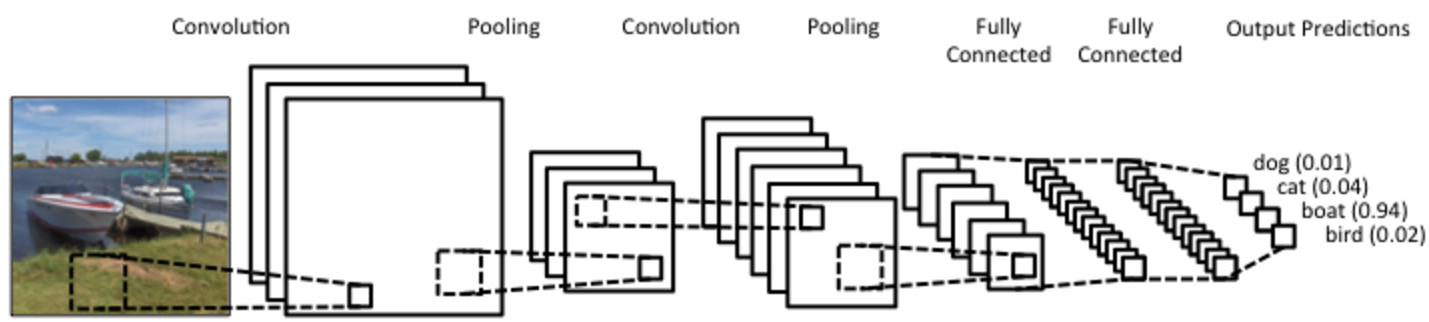
\includegraphics[width=0.9\textwidth]{bilder/cnn_overview.png}
	\caption{Schematic overview of a CNN architecture. \hspace{\textwidth}
		\tiny (Image from https://medium.com/@Aj.Cheng/convolutional-neural-network-d9f69e473feb, 12.05.2018)}
	\label{fig:cnn_overview}
	\end{figure}
\end{frame}

\begin{frame}
	\frametitle<presentation>{Convolution (in images)}
	\begin{figure}[!t]
	\centering
		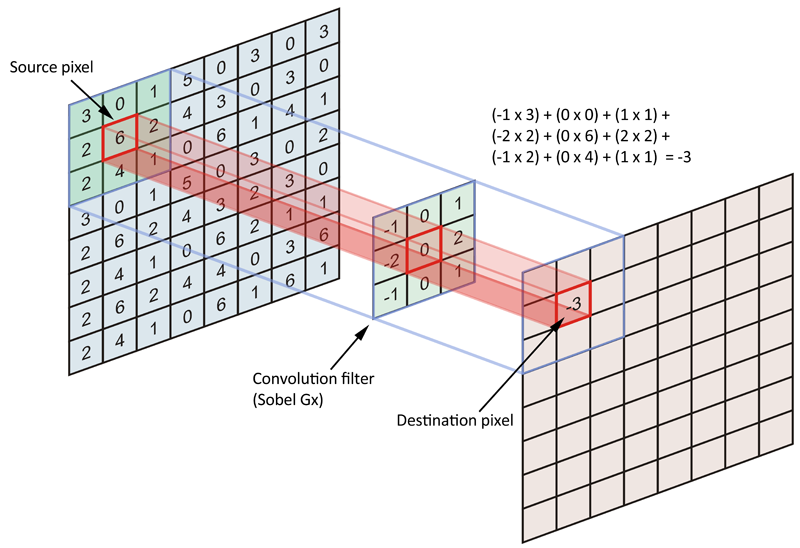
\includegraphics[width=0.5\textwidth]{bilder/convolution.png}
	\caption{2D-convolution: weighted sum over a local patch of data. \hspace{\textwidth}
		\tiny (Image from https://i.stack.imgur.com/YDusp.png, 12.05.2018)}
	\label{fig:convolution}
	\end{figure}
	\note[item]{As the name suggests, the most important parts of a CNN are the convolutional layers. In these layers the whole input is processed by convolutional filters that output a feature map.}
	\note[item]{Convolution (in images) is basically just a weighted sum over a local patch of data as you can see here.}
	\note[item]{A lot of classical image processing is done by using convolutional matrices. Depending on the weights and size of the filter you can extract different information from the images.}
	\note[item]{Here, for example, is a filter that extracts gradients in the x-direction in an image, so it is basically an edge filter for vertical edges.}
	\note[item]{These filters are usually pre-defined by the inventor or developer of a certain algorithm and dont change}
	\note[item]{In CNNs however, these filters or the weights in the matrices are learned by the computer.}
\end{frame}
 

\section{Proposed Method}

\subsection{Architecture}

\begin{frame}
	\frametitle<presentation>{Architecture}
	\begin{itemize}
		\item BraTS 2013 dataset.
		\note[item]{ BraTS: Brain Tumor Segmentation \\
			competition where research teams evaluate their algorithms, similar to ImageNet}
		\item Slice by slice segmentation due to bad depth resolution.
		\note[item]{They perform the segmentation slice by slice, so the segmentations of each layer in the dataset dont influence each other}
		\item Different image modalities of the same structures.
	\end{itemize}
	\begin{figure}[!t]
		\centering
			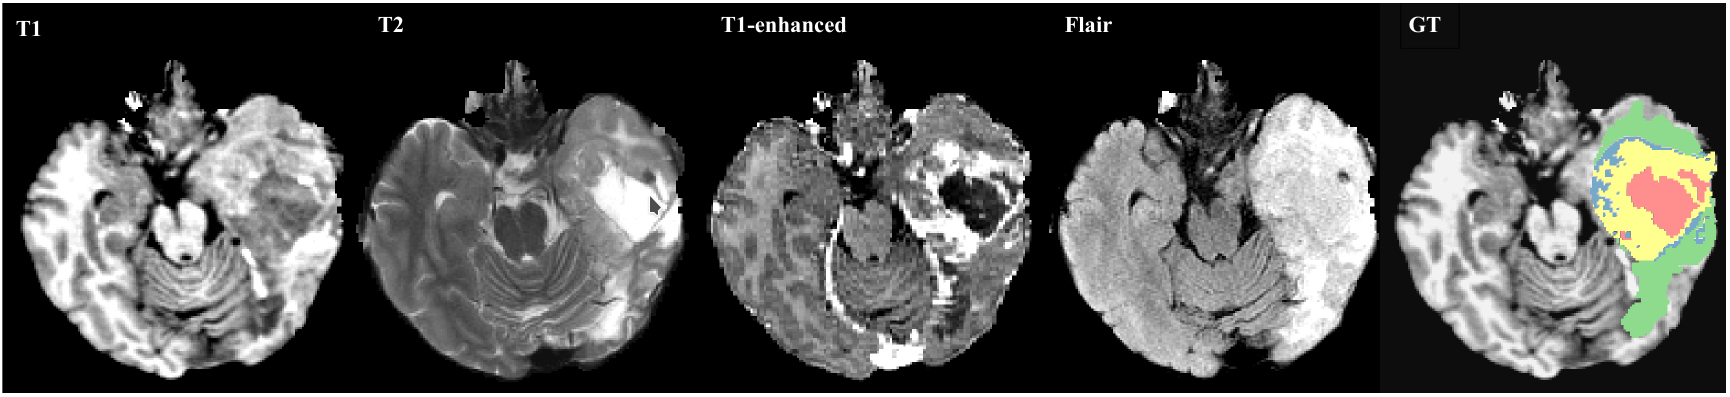
\includegraphics[width=\textwidth]{bilder/mri_sequences.png}
		\caption{MRI sequences used as input channels and ground truth labels (p. 9, figure 4).}
		\label{fig:mri_sequences}
	\end{figure}
\end{frame}

\begin{frame}
	\frametitle<presentation>{Architecture}
	\note[item]{They evaluated different architectures, so basically different setups of convolutional and other layers.}
	\note[item]{First, they developed a small CNN that processes the input data in two different paths: ...}
	\note[item]{Then, in their so-called 'cascaded architectures' they put two of those smaller CNNs together in order to model dependencies between spatially close labels. We will see in a minute what that means exaclty ...}
	\begin{block}{Two-pathway architecture:}
		\begin{itemize}
			\item One smaller ($7 \times 7$) and one larger ($13 \times 13$) receptive field.
			\item Prediction based on local region and larger context.
		\end{itemize}
	\end{block}
	\begin{block}{Cascaded architectures:}
		\begin{itemize}
			\item Goal: model dependencies between spatially close labels by
			\item \emph{input concatenation},
			\item \emph{local pathway concatenation}, and
			\item \emph{pre-output concatenation}.
		\end{itemize} 	
 	\end{block}
\end{frame}

\begin{frame}
	\frametitle<presentation>{Two-pathway architecture}
	\note[item]{In the two-pathway architecture they take a 4x33x33 input patch (4 for the four different image modalities) and propagate the patch through two independent paths of their network.}
	\note[item]{Their main difference are the different receptive fields of the first convolutional layer. In one layer they process the image with a larger convolutional matrix than in the other}
	\note[item]{At the end they simply concatenate the different feature maps of the two paths and perform the final evaluation of the pixel labels on the data of both.}
	\begin{figure}[!t]
		\centering
			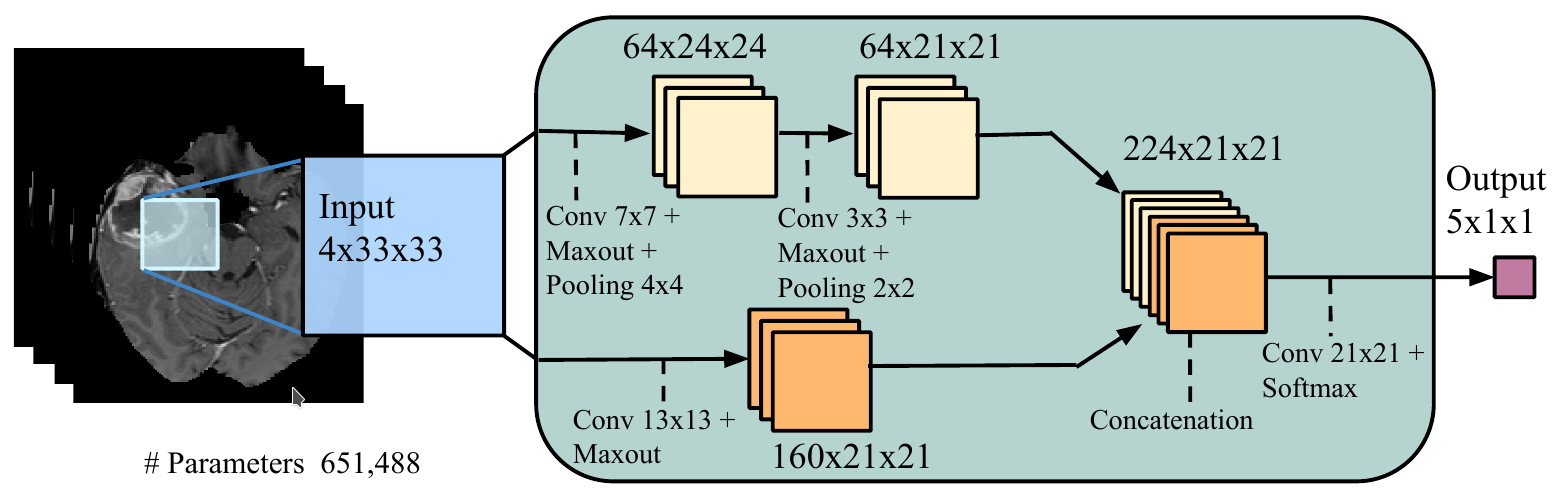
\includegraphics[width=\textwidth]{bilder/two_pathway.png}
		\caption{Two-pathway CNN architecture (p. 6, figure 2).}
		\label{fig:two_pathway}
	\end{figure}
\end{frame}

\begin{frame}
	\frametitle<presentation>{Cascaded architecture}
	\note[item]{In the cascaded architectures, they take the CNN from before, but add to that a second version of it with a slightly different input patch.}
	\note[item]{Explain...}
	\begin{figure}[!t]
		\centering
			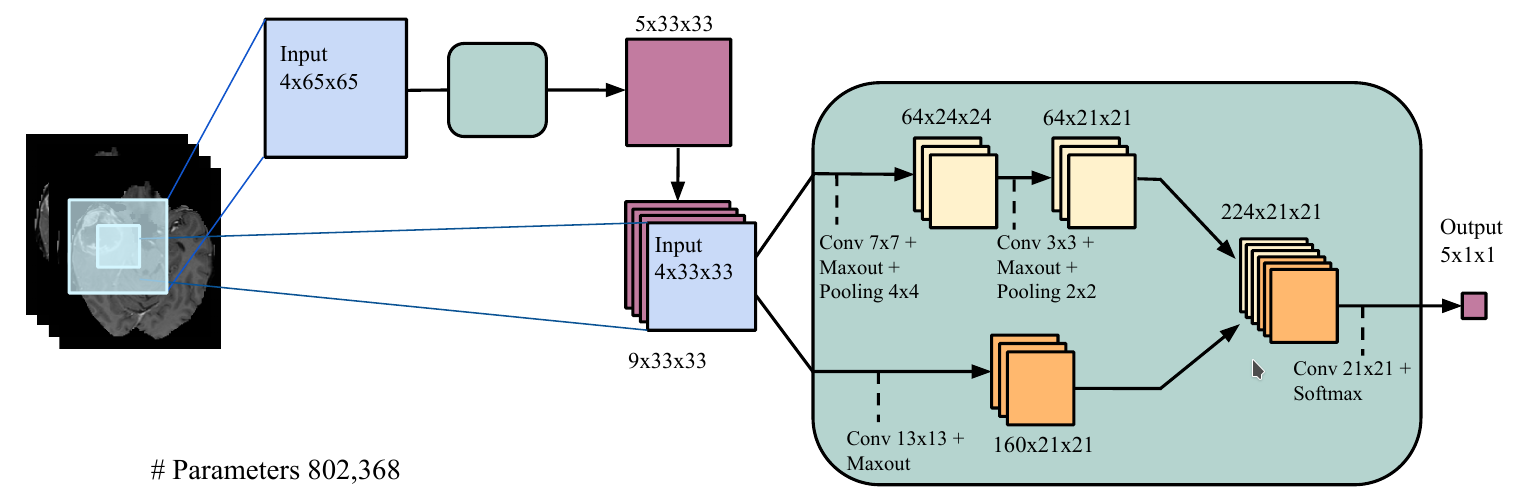
\includegraphics[width=\textwidth]{bilder/cascade1.png}
		\caption{Cascaded architecture using input concatenation to combine two CNNs (p. 7, figure 3).}
		\label{fig:cascade1}
	\end{figure}
	\note[item]{Shown: Input concatenation}
	\note[item]{Also tested: Local pathway concatenation, pre-output concatenation}
	\note[item]{So, essentially, they take the labels from one CNN and use it as an additional input for a second CNN that uses the original image data and the label probabilities of the surrounding area. That way they model the dependencies of each label to one another.}
\end{frame}

\subsection{Training}

\begin{frame}
	\frametitle<presentation>{Training}
	\begin{block}{Gradient Descent:}
		\begin{itemize}
			\item Forward propagation on a mini-batch of patches.
			\item Compute label probabilities and deviation from ground truth.
			\item Update the CNNs parameters.
		\end{itemize}
	\end{block}
	\begin{block}{Two-phase training:}
		\begin{itemize}
			\item Highly imbalanced data ($98 \%$ healthy voxels).
			\note[item]{Selecting patches from true distribution causes problems}
			\item First: Pick patches such that all labels are equiprobable.
			\item Then: Re-train output layer with original distribution.
			\note[item]{Best of both worlds: First step makes the filters sensitive to the searched features\\
				Second step calibrates the output probabilities correctly}
		\end{itemize} 	
 	\end{block}
 	\begin{block}{Regularization:}
		\begin{itemize}
			\item Prevent overfitting by bounding kernel weights and modifying output probabilities.
			\note[item]{Modify output probabilities with factors that encourage sparsity and small values in kernels (high values lead to unstable gradients for example)}
		\end{itemize} 	
 	\end{block}
 	\note[item]{Mention training of cascaded architectures... train two path first, then fix parameters}
\end{frame}

\subsection{Results}

\begin{frame}
	\frametitle<presentation>{Two-pathway architecture}
	\begin{itemize}
		\item Second phase and joint training of local and global path yields better performance.
		\item Very fast, about 25s for a whole brain.
		\note[item]{The methods with the appended asterisk here are the methods that used the two-phase training I have mentioned before}
		\note[item]{200 times faster than the winner of the challenge (100m)}
		\note[item]{Other methods range between 6 and 90 minutes}
	\end{itemize}
	\begin{table}
		\caption{Quantitative results of the two-pathway architecture variations on the BRATS 2013 dataset, where the appended * denotes two-phase training (p. 11, table 1).}
		\label{tab:beispiel}
		\centering
			\begin{tabular}{ccccc}
				\toprule
				Rank & Method & Dice & Specifity & Sensitivity \\
				\midrule
				4 	& TwoPathCNN* 		& 0.85	& 0.93	& 0.80\\
				9 	& LocalPathCNN* 		& 0.85	& 0.91	& 0.80\\
				10 	& AverageCNN* 		& 0.84	& 0.95	& 0.77\\
				14 	& GlobalPathCNN* 	& 0.82	& 0.93	& 0.75\\
				14 	& TwoPathCNN 		& 0.78	& 0.67	& 0.96\\
				15 	& LocalPathCNN		& 0.77	& 0.65	& 0.96\\
				\bottomrule
			\end{tabular}
	\end{table}
\end{frame}

\begin{frame}
	\frametitle<presentation>{Cascaded architecture}
	\begin{itemize}
		\item Fast, about 3 minutes for a whole brain.
		\item Winner of the challenge takes about 100 minutes.
		\note[item]{30 times faster than winner of the challenge (100m)}
		\note[item]{Other methods range between 6 and 90 minutes}
	\end{itemize}
	\begin{table}
		\caption{Quantitative results of the cascaded architecture variations on the BRATS 2013 dataset, where the appended * denotes two-phase training (p. 13, table 2).}
		\label{tab:beispiel}
		\centering
			\begin{tabular}{ccccc}
				\toprule
				Rank & Method & Dice & Specifity & Sensitivity \\
				\midrule
				2 	& InputCascadeCNN*	& 0.88	& 0.89	& 0.87\\
				4-a & MFCascadeCNN* 		& 0.86	& 0.92	& 0.81\\
				4-b & LocalCascadeCNN* 	& 0.88	& 0.91	& 0.84\\
				\bottomrule
			\end{tabular}
	\end{table}
\end{frame}

\begin{frame}
	\frametitle<presentation>{Cascaded architecture}
			\note[item]{Here is an example of one slice of the dataset, its ground truth data and the CNNs segmentation output after different phases of learning.}
			\note[item]{As you can see, in the first phase, the general look of the segmentation looks okay, but there are still a lot of wrong labels, because the net assumes an equal distribution of the different kinds of pixels.}
			\note[item]{This changes in the second phase where the CNN is refined with the original data and eventually you get a pretty good result... }
	\begin{figure}[!t]
		\centering
			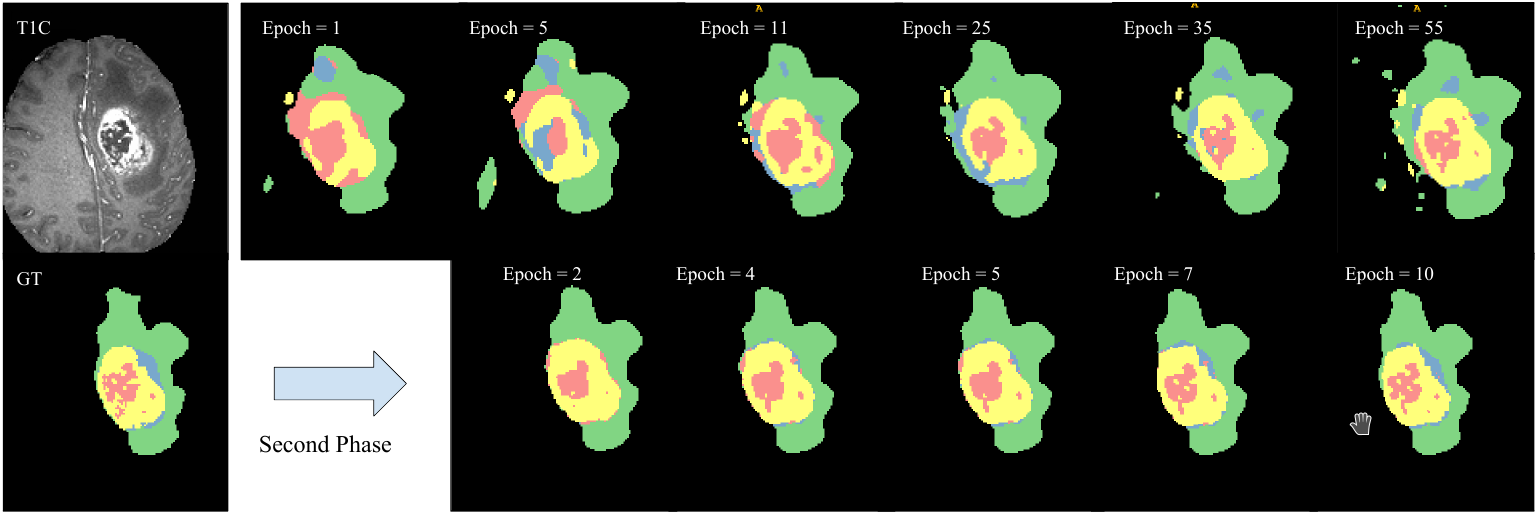
\includegraphics[width=\textwidth]{bilder/input_cascade.png}
		\caption{Progression of learning InputCascadeCNN* (p. 11, figure 6).}
		\label{fig:cascade1}
	\end{figure}
\end{frame}

\section{Conclusion}

% nur für die Miniframe-Navigation
\subsection*{}

\begin{frame}
	\frametitle<presentation>{Conclusion}
	\begin{itemize}
  		\item Automatic brain tumor segmentation based on deep learning (Convolutional Neural Networks).		
	\end{itemize}	
	\vfill
	\begin{block}{Improve on currently published state-of-the-art methods}
		\begin{itemize}
			\item Improvements especially in speed (25s to 3m per brain).
		\end{itemize}
	\end{block}
	\begin{block}{Novel two-pathway architecture}
		\begin{itemize}
			\item Fuse local details and global context.
			\item Model local dependencies of labels.
		\end{itemize} 	
 	\end{block}
 	\note[item]{So, to summarize everything I have told you:}
 	\note[item]{The group developed an automatic brain tumor segmentation method based on Convolutional Neural Networks}
 	\note[item]{They improved on a lot of other published methods of that time or got at least similar results, but with a lot less computational effort.}
 	\note[item]{They have achieved this with their novel two-pathway architecture:}
 	\note[item]{With that they are able to fuse local details as well as the pixel's global context and they used concatenation of feature maps to model local dependencies for the different labels.}
\end{frame}

% nur für die Miniframe-Navigation
\section*{}

\begin{frame}<beamer>{}
	\begin{center}
		Thank you for your attention!
	\end{center}
	\begin{center}
		Any questions?
	\end{center}
\end{frame}

\begin{frame}
	\frametitle<presentation>{Additional information}
	\begin{block}{Imbalanced data}
		\begin{itemize}
			\item Assume a predictor trained on 10 malignant and 90 benign tumors. A model could predict "benign" for all samples and still gain a very high accuracy. An unbalanced dataset will bias the prediction model towards the more common class!
		\end{itemize}
	\end{block}
	\begin{block}{Gradient Descent}
		\begin{itemize}
			\item Maximize the probability of all labels in the training set or, equivalently, minimize the negative log-probability for the label $\mathbf{Y}$ given the data $\mathbf{X}$:
		\end{itemize}
	\begin{equation}
		 -\log p(\mathbf{Y}|\mathbf{X}) = \sum\limits_{ij} -\log p(Y_{ij}, \mathbf{X})
	\end{equation}
	\end{block}	
\end{frame}

\begin{frame}
	\frametitle<presentation>{Additional information}
	\begin{block}{Quantitative Measurements}
		\begin{equation}
			Dice(P, T) = \frac{2 |P_1 \cap T_1|}{|P_1| + |T_1|}
		\end{equation}
		\begin{equation}
			Sensitivity(P, T) = \frac{|P_1 \cap T_1|}{|T_1|}
		\end{equation}
		\begin{equation}
			Specificity(P, T) = \frac{|P_0 \cap T_0|}{|T_0|}
		\end{equation}
		\begin{itemize}
			\item $P$ - model predictions
			\item $T$ - ground truth
			\item Index 1 for positives and index 0 for negatives for the tumor region in question
		\end{itemize}
	\end{block}
\end{frame}

\end{document}\grid
\grid
